% !TEX root =..\main.tex
\section{ТЕОРЕТИЧЕСКИЙ АНАЛИЗ}

    \subsection{Анализ существующего прототипа на движке Citrus}

        В ходе курсовой работы был создан прототип двухмерной игры на движке Citrus Engine. Задачи прототипа включали: отображение анимации персонажа, 
        обработку пользовательского ввода, взаимодействие с сервером и отрисовку обновленного игрового состояния, обработку голосового потока и преобразование его в текст,
        а также генерацию голосового ответа для игрока. Игровой мир состоял из тайловых карт, загружаемых из текстовых файлов и набора спрайтов для визуализации окружающей среды и объектов.
        
        \subsubsection{Архитектура прототипа}

        В основе прототипа лежит клиент-серверная архитектура с выделенным модулем распознавания команд, модулем распознавания речи (ASR) и модулем синтеза речи (TTS). 
        Все компоненты взаимодействуют в рамках игрового цикла, обеспечивая прием голосовых команд от пользователя, их интерпретацию в игровые действия, 
        обновление состояния и обратную отдачу в виде визуального и звукового ответа. Основные блоки системы:

        \textbf{Клиентская часть}
        
        Отвечает за сбор голосового ввода от пользователя, передачу аудиопотока на сервер, десериализацию и отображение обновлённого игрового состояния. 
        После получения от сервера готовых данных клиент одновременно рендерит игровые объекты и воспроизводит аудиоответ.

        \textbf{Основной серверный процесс}
        
        Вся серверная часть контролируется основным процессом. При его запуске, в отдельном потоке инициализируются все модули проекта, а также
        в консоль выводится детальная информация о состоянии модулей с помощью библиотеки Terminal.Gui.
        \begin{lstlisting}[caption=Инициализация модулей]
var gameLoopThread = new Thread(GameLoop);
var networkThread = new Thread(NetworkLoop);
var broadcastThread = new Thread(BroadcastLoop);
var consoleThread = new Thread(ConsoleLoop);
var voiceEmitterThread = new Thread(VoiceEmitterLoop);
var voiceRecognitionTask = new Task(VoiceRecognitionLoop);
        \end{lstlisting}

        \textbf{Модуль распознавания команд}
        
        Принимает непрерывный аудиопоток от клиента, отправляет его на обработку в модуль ASR, 
        получает распознанный текст, затем преобразует его в формализованную игровую команду и передаёт на сервер.
        Список возможных команд продемонстрирован в таблице в \textbf{приложении Г}.

        \textbf{Модуль игровой логики}

        Получив игровую команду, сервер обновляет игровое состояние (положение юнитов, их здоровье и т.д.) и формирует один или 
        несколько объектов TaskResult, описывающих результаты действия (перемещение юнита, изменение ресурсов, возникновение событий и т. д.).
        Эти объекты передаются в очередь модуля TTS для дальнейшего синтеза аудиоответа. Одновременно с этим обновленное игровое состояние
        сериализуется, затем посредством библиотеки LiteNetLib и сетевого протокола UDP передается на клиент.

        \textbf{Модуль Text-to-Speech}
        
        Извлекает объект TaskResult из очереди и на его основе с помощью алгоритма синтеза речи генерирует аудиопоток с голосовым сообщением игр
        отправляет его на клиент по протоколу gRPC.

        \textbf{Канал возврата данных}
        
        Игра и модуль TTS завершают такт независимо: сервер отправляет клиенту обновлённое состояние, а TTS -- аудиопоток ответа. 
        Клиент обрабатывает оба результата <<по приходу>>, синхронно обновляя интерфейс и воспроизводя голосовое сообщение.
        

        \begin{figure}[H]
            \centering
            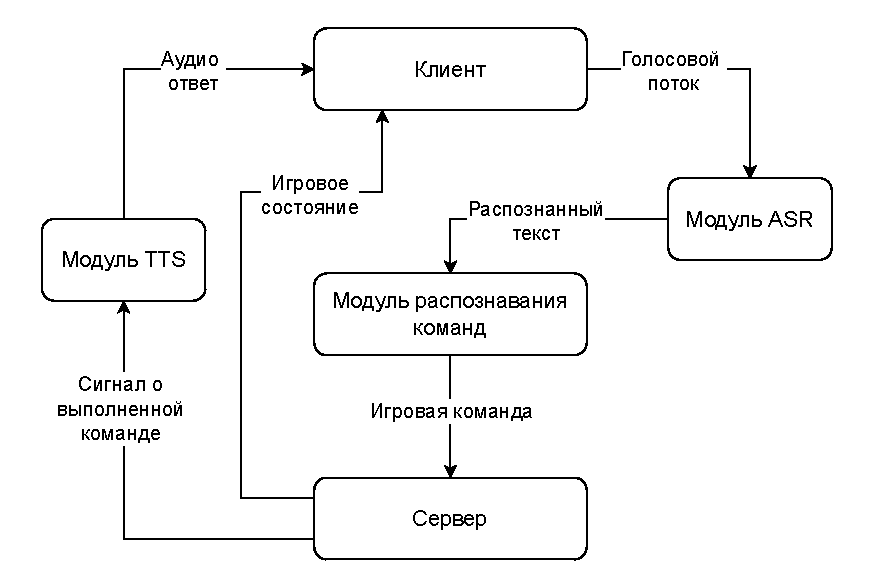
\includegraphics[scale=1]{pictures/architecture_scheme.pdf}
            \caption{Блок-схема архитектуры}\label{ris1.1}
        \end{figure}

        Такая архитектура (рисунок \ref{ris1.1}) позволяет гибко масштабировать голосовой интерфейс и логику игры, развивая каждый модуль отдельно: оптимизировать ASR-движок, улучшать логику генерации 
        TaskResult или внедрять новые голоса в TTS, не затрагивая остальные компоненты.

        \subsubsection{Игровой цикл}

        Игровой цикл прототипа можно свести к следующим этапам:

        \begin{itemize}
            \item пользователь на клиенте произносит голосовую команду;
            \item клиент шлёт аудиопоток на сервер, где модуль распознавания команд совместно с языковой моделью преобразует звук в текст и переводит его в формальную игровую команду;
            \item серверный игровой движок принимает команду, изменяет состояние и создаёт объекты TaskResult;
            \item тaskResult передаётся в модуль TTS, который синтезирует аудиоответ; одновременно обновлённое игровое состояние возвращается клиенту как отдельный пакет;
            \item клиентская часть отображает новый кадр игры и воспроизводит полученный голосовой ответ.
        \end{itemize}

        
        \subsubsection{Технические и организационные проблемы Citrus}

        В процессе разработки прототипа на Citrus стало ясно, что дальнейшее расширение проекта на этой платформе встретит серьёзные затруднения: сама экосистема 
        движка жёстко завязана на Windows, что исключает возможность экспорта приложения под Linux, macOS или мобильные устройства, а попытки 
        обойти это ограничение требуют непропорционально больших усилий и рисков несоответствия требованиям целевых платформ. Кроме того, официальная документация сводится 
        лишь к перечню классов и методов без каких-либо практических рекомендаций по построению архитектуры или описания сложных сценариев работы, поэтому разработчикам 
        приходится изучать движок эмпирическим путем, додумывая что делает тот или иной метод. Внутренняя организация движка избыточно детализирована и сильно загромождена кодом: 
        вместо того чтобы предоставить разработчику готовые, высокоуровневые абстракции для ввода-вывода, анимации и рендеринга, Citrus вынуждает 
        разбираться с низкоуровневыми реализациями и вручную настраивать связи между модулями. При этом отсутствуют 
        специализированные библиотеки или готовые плагины, которые могли бы взять на себя обработку ввода с контроллеров и клавиатуры, проигрывание сложных анимационных 
        последовательностей или оптимизированный отрисовочный конвейер, поэтому любую подобную функциональность приходится реализовывать самостоятельно поверх уже громоздкой, 
        неинтуитивной структуры движка. Постоянная необходимость вручную синхронизировать многочисленные файлы и конфигурации усложняет 
        сопровождение кода и практически исключает автоматизированный рефакторинг, а отсутствие активного сообщества, форумов, учебных курсов и открытых примеров практически 
        обесценивает любые усилия по поиску готовых решений или обмену опытом: каждый новый вопрос превращается в многодневный эксперимент, что полностью нивелирует преимущество 
        быстрой прототипизации.

        Все эти факторы делают дальнейшую разработку крупного или коммерчески значимого проекта на Citrus нецелесообразной. Для обеспечения кроссплатформенности, простоты поддержки 
        и быстрой интеграции необходимых модулей требуется смена движка.

    \subsection{Сравнительный анализ технологий}

        \subsubsection{Игровые движки}

        \textbf{Критерии выбора нового движка}

        При выборе альтернативного движка учитывались следующие критерии:
        \begin{itemize}
            \item поддержка языка программирования C\# (Поскольку существенная часть кода прототипа была написана именно на этом языке);
            \item кроссплатформенность (Windows, Linux, мобильные платформы);
            \item наличие и полнота документации, обучающих материалов, примеров;
            \item развитое сообщество и экосистема (Библиотека ассетов, плагины, расширения);
            \item простая и гибкая архитектура проектов (удобная структура сцен/сценариев, минимальная настройка конфигурационных файлов).
        \end{itemize}


        \textbf{Сравнение движков}

        \textbf{Citrus}

        Citrus -- игровой движок российской компании Game Forest, предназначенный для разработки 2D игр, 
        разрабатывающийся для внутреннего пользования, однако, также присутствует публичная версия. Поскольку он находится на ранних этапах разработки, 
        у него отсутствуют какие-либо справочные материалы, помимо плохо составленной документации. Также присутствует редактор сцен, который никак не 
        задокументирован, а его нагроможденность делает его практически бесполезным. Несмотря на это, он все же пригоден для создания игр, 
        но для разработчика, не имеющего отношения к этой компании, это будет весьма затруднительно. Вместе с движком предоставляются примеры готовых проектов 
        в жанре "платформер" и "3 в ряд" для ознакомления с его функционалом, однако, этого недостаточно для комфортной разработки RTS.

        \textbf{Unity}

        Unity давно зарекомендовал себя эталоном кроссплатформенной разработки: редактор доступен на Windows и macOS, экспорт проектов поддерживается на все актуальные настольные 
        операционные системы, iOS, Android и даже игровые консоли. Официальная документация Unity включает полные справочники API, пошаговые руководства, 
        обучающие видео и обширную базу примеров, что позволяет быстро освоиться как начинающим, так и опытным разработчикам. Развитое сообщество вокруг Unity гарантирует 
        наличие тысяч готовых плагинов и ассетов в Asset Store, регулярные обновления движка и ответы на наиболее частые вопросы на форумах и в тематических чатах. Архитектура проектов 
        в Unity строится вокруг концепции сцен и префабов (Prefabs): сцены организуются в упорядоченную и понятную иерархию игровых объектов, а конфигурационные файлы сведены к минимуму, 
        поскольку большая часть настроек хранится в самих префабах. Наконец, поддержка языка C\# является одной из сильных сторон Unity: весь пользовательский код пишется 
        именно на нём, что позволяет без портирования переиспользовать значительную часть логики из прототипа.
        
        \textbf{Unreal Engine}

        Unreal Engine демонстрирует хорошую кроссплатформенность на уровне экспорта -- проекты могут быть собраны под Windows, macOS, Linux, Web через Pixel Streaming, а также на 
        мобильные платформы и консоли. Документация Unreal отличается глубиной технических объяснений, однако основной упор сделан на C++ и визуальные скрипты Blueprint. 
        Сообщество Unreal велико, имеет собственный магазин ассетов и множество учебных курсов, но в сфере 2D-игр движок нередко воспринимают как <<тяжёлый>> и избыточный. 
        Архитектура проектов в UE сложнее: уровни, акторы, компоненты и классы C++ формируют мощную, но громоздкую структуру, требующую детального понимания внутренней логики движка. 
        Что касается C\#, официальной интеграции нет -- подобные возможности реализуются лишь через сторонние плагины и зачастую сопровождаются высокой затратой времени на настройку.
        
        \textbf{Godot}

        Godot представляет собой полностью свободный движок с редактором на Windows, Linux и macOS и универсальным экспортом под все популярные платформы, включая Web и мобильные ОС. 
        Документация Godot охватывает как справочник API, так и пошаговые гайды по разработке, а активное и быстро растущее сообщество регулярно публикует готовые демо-проекты и видеоуроки. 
        Встроенная Asset Library постепенно наполняется шаблонами и расширениями, хотя пока не достигает масштабности Unity Asset Store, но для 2D-игр базового набора достаточно.
        Проектная архитектура Godot основана на лёгкой и гибкой системе сцен и узлов: вместо многочисленных конфигураций создаются сцены, вложенные в другие сцены, и настраиваются связи 
        прямо в визуальном редакторе. Это позволяет быстро прототипировать и при этом легко масштабировать проект. Начиная с версии 3.x, Godot имеет полноценную поддержку C\# под управлением 
        Mono: код на C\# компилируется и выполняется наряду с GDScript, что облегчает перенос и развитие написанной ранее логики.

        \begin{table}[ht]
            \caption{Сравнение игровых движков}
            \centering
            \renewcommand{\arraystretch}{1.2}
            \renewcommand{\tablename}{Табл.}
            \begin{tabularx}{\textwidth}{|X|X|X|X|X|X|}
            \hline
            &\textbf{Поддержка C\#} & \textbf{Кросспла-тформенн-ость} & \textbf{Подробная документация} & \textbf{Размер сообщества} & \textbf{Простота освоения} \\
            \hline
            Citrus&Да&Нет&Нет& Нулевой&Тяжело\\
            \hline
            Unity&Да&Да&Да& Большой&Умеренно\\
            \hline
            Unreal&Нет&Да&Да&Большой&Очень тяжело\\
            \hline
            Godot&\textbf{Да}&Да&\textbf{Да}&Средний&\textbf{Легко}\\
            \hline
            \end{tabularx}
        \end{table}

        При сравнительной оценке по пяти ключевым критериям Unity и Godot отвечают всем требованиям: Unity выигрывает за счёт зрелости экосистемы и количества готовых решений, 
        Godot привлекает открытостью, лёгкостью проекта и достаточной поддержкой C\#. Unreal Engine, хотя и силён в 3D-разработке, не оптимален для C\#-ориентированной 2D-игры. 
        Учитывая баланс между простотой использования, быстрой кроссплатформенной сборкой, обилием документации и непосредственной поддержкой C\#, окончательным выбором стал Godot Engine.

        С переходом на Godot открывается целый набор средств для быстрой и гибкой доработки геймплея и интерфейса. Его система сцен и узлов позволяет 
        создавать многослойный HUD: Control-узлы и CanvasLayer и Control легко организуют главное меню, окно управления юнитами и всплывающие подсказки, 
        а встроенные Theme-ресурсы (StyleBox, Font) обеспечивают единый стиль и адаптивную вёрстку под разные разрешения экрана. Во-вторых, визуальный конвейер Godot 
        поддерживает 2D-шейдеры, благодаря чему <<туман войны>> можно реализовать прямо на GPU.

        Кроме того, сцены-шаблоны облегчают добавление новых игровых объектов и элементов пользовательского интерфейса: через наследование или композицию можно разграничить общие параметры 
        и уникальные скрипты поведения. Полноценная поддержка C\# и «горячая» перезагрузка скриптов (hot reload) сокращают время отладки: изменения в коде вступают в силу мгновенно, 
        без перезапуска игрового клиента, а кроссплатформенный экспорт (Windows, Linux, macOS, Android, iOS) позволяет сразу проверять поведение и производительность на любых целевых устройствах.

        Благодаря таким возможностям внедрение классических RTS-элементов станет удобным и оперативным: новые игровые объекты будут конфигурироваться визуально, а программная логика 
        останется сосредоточенной в читаемом и легко поддерживаемом коде. Вместо ручного переписывания низкоуровневых компонентов, появится возможность сфокусироваться на дизайне 
        баланса, сценариях развития игроков и качественном тестировании механик, что значительно ускорит трансформацию прототипа в полнофункциональную стратегию.

        \subsubsection{Сетевые архитектуры}

        В контексте разработки многопользовательских сетевых игр обычно применяют один из трех основных подходов: peer-to-peer, клиент-серверную архитектуру и гибридные решения. Ниже приведет краткий 
        обзор их сильных и слабых сторон:

        \textbf{Peer-to-Peer (P2P)}

        В P2P-сети каждый игрок напрямую обменивается сообщениями с остальными участниками. Такой подход позволяет избавиться от необходимости разработки серверной части 
        и минимизировать задержки при передаче команд, поскольку обмен пакетов происходит напрямую между игроками, однако для RTS-игр это требует строгой детерминированности игрового 
        движка (чтобы все клиенты, получив одни и те же команды, гарантированно пришли к одному и тому же состоянию мира) и сложной системы синхронизации (lockstep). Кроме того, 
        P2P-сети плохо масштабируются при большом числе участников и уязвимы к читерским вмешательствам. Дополнительно от клиента потребуются вычислительные мощности, чтобы распознавать текст
        из аудиопотока и синтезировать аудиоответ.
        
        \textbf{Клиент-серверная}

        Все действия игроков проходят через единый сервер, который проверяет валидность команд, обновляет состояние мира и рассылает клиентам результат. 
        Такой подход исключает необходимость в детерминированном движке, упрощает борьбу с читерством и централизует логику синхронизации. Сервер, обрабатывая запросы на управление 
        (в том числе текстовые команды из ASR), может дополнительно валидировать их через синтаксический разбор, фильтровать «спам» голосовых запросов и шифровать трафик. Выбор 
        клиент-серверной архитектуры для сетевой RTS обоснован следующими факторами. Во-первых, голосовые команды должны распознаваться и интерпретироваться однозначно: централизованный 
        сервер с ASR-модулем (Vosk) и языковой моделью позволяет гарантировать единообразие обработки, быстрее вносить правки в модель команд и собирать статистику ошибок. Во-вторых, хранение 
        и управление состоянием игры на сервере упрощает защиту от читерства (нельзя напрямую отправить на клиент некорректную команду) и делает возможным масштабирование: при росте числа игроков 
        достаточно добавить новые экземпляры серверного кластера с балансировкой нагрузки. В-третьих, централизованное решение позволяет интегрировать модуль TTS на серверной стороне 
        и выдавать клиентам синхронизированный аудио- и графический отклик без рассинхронизации, которая обычно возникает в P2P-сетях. Наконец, клиент-серверная модель лучше вписывается 
        в сценарии кроссплатформенной сборки на Godot и C\#: серверная часть может работать на хосте с мощным <<железом>> с выделенным ASR/TTS, а клиенты на любых устройствах лишь получают 
        финальные пакеты.
        
        \textbf{Гибридные архитектуры}

        Комбинируют элементы P2P и клиент-серверной моделей: например, авторитетный сервер только реплицирует важные события, а менее критичные данные 
        передают напрямую между клиентами. Это позволяет частично разгрузить сервер и уменьшить задержки, но резко усложняет логику: приходится одновременно поддерживать два протокола 
        взаимодействия, делать дополнительную защиту целостности данных и обрабатывать рассинхронизации.

        \begin{table}[ht]
            \caption{Сравнение сетевых архитектур}
            \centering
            \begingroup
            \fontsize{12}{14}\selectfont
            \renewcommand{\arraystretch}{1.2}
            \renewcommand{\tablename}{Табл.}
            \begin{tabularx}{\textwidth}{|X|X|X|X|X|}
            \hline
            \textbf{Движок}&\textbf{Централизова-нность} & \textbf{Задержка} & \textbf{Необходимость сервера}&\textbf{Простота синхронизации}\\
            \hline
            P2P&Нет&Минимальная&Нет&Тяжело\\
            \hline
            Клиент-серверная&\textbf{Да}&Средняя&Да&\textbf{Легко}\\
            \hline
            Гибридная&Частично&Средняя&Да&Умеренно\\
            \hline
            \end{tabularx}
            \endgroup
        \end{table}
        
        Таким образом, клиент-серверный подход обеспечивает оптимальный баланс между надёжностью, безопасностью, простотой синхронизации и расширяемостью архитектуры.

        \subsubsection{ASR-решения}

        К ASR модулю были выставлены следующие требования:
        \begin{itemize}
            \item поддержка русского языка на достойном уровне точности (word error rate (WER) $\leq$ 10 \%);
            \item наличие C\#-библиотеки;
            \item возможность работы в офлайн-режиме для снижения задержек;
            \item умеренные требования к ресурсам сервера (CPU, память).
        \end{itemize}

        При выборе системы автоматического распознавания речи для серверной части сетевой RTS оценивались как локальные движки, так и облачные сервисы. Наиболее подходящим локальным решением оказался 
        Vosk -- это обёртка над библиотекой Kaldi с уже готовыми моделями для русского языка и официальной C\#-библиотекой Vosk.CSharp. При тестировании Vosk на сервере с четырьмя ядрами и 8 ГБ 
        памяти средний WER (word error rate) держался на уровне 6-8 \%, а End-to-End задержка от получения пакета до выдачи текста 
        состав­ляла порядка 80–120 мс. Благодаря офлайн-режиму Vosk не зависит от качества канала связи и не генерирует дополнительных расходов, что делает его особенно привлекательным для 
        сетевых игр с высокой нагрузкой.

        В противоположность локальным движкам, облачный Yandex SpeechKit впечатлил более низким WER (в районе 4–5 \%) даже в условиях фонового шума, однако реальная задержка при обмене
        аудиопакетами через HTTPS достигала 150–200 мс. При этом стоимость распознавания в Yandex Cloud оценивается по количеству минут, и при прогнозируемом игровом трафике она бы превысила
        все доступные для студенческого проекта бюджеты. Кроме того, зависимость от облака вводила риск снижения качества голосового интерфейса при любой нестабильности интернет-соединения. 
        В итоге облачный вариант тестировался лишь в демонстрационных целях, но для финальной версии пришлось от него отказаться в пользу полностью локального решения.

        Среди альтернатив рассматривались DeepSpeech от Mozilla и Whisper от OpenAI. DeepSpeech при использовании русскоязычных моделей показывает более высокий WER (около 10–12 \%) и большую 
        задержку -- 150–200 мс на аналогичном железе, а официальной поддержки .NET у проекта нет, поэтому интеграция требовала бы самостоятельной сборки нативных библиотек и создания C\#-обёртки. 
        Whisper отличается отличной точностью (WER примерно 3–5 \%), но требует наличия GPU-ускорения и приличных оперативных ресурсов (минимум 4–8 ГБ видеопамяти) для работы в реальном времени, 
        а также на сегодня не имеет C\#-библиотек.


        \begin{table}[ht]
            \caption{Сравнение ASR решений}
            \centering
            \renewcommand{\arraystretch}{1.2}
            \renewcommand{\tablename}{Табл.}
            \begin{tabularx}{\textwidth}{|X|X|X|X|X|}
            \hline
            \textbf{Решение} & \textbf{WER, \%} & \textbf{Задержка, мс} & \textbf{C\#-SDK} & \textbf{Офлайн-режим} \\
            \hline
            Vosk&6–8&80–120&Да&Да \\
            \hline
            Yandex SpeechKit&<5&150–200&Да&Нет \\
            \hline
            DeepSpeech&10–12&150–200&Нет&Да\\
            \hline
            Whisper&3–5&200–300&Нет&Да\\
            \hline
            \end{tabularx}
        \end{table}

        Таким образом, учитывая ключевые требования -- качественное распознавание русского, готовый C\#-SDK и офлайн-режим без дополнительных затрат -- выбор пал на Vosk. 
        Он позволяет управлять нагрузкой и не привязывает проект к внешним сервисам, что обеспечивает стабильность игрового процесса и предсказуемость задержек при передаче голосовых команд.

        \subsubsection{TTS-решения}

        При выборе движка синтеза речи основной упор делался на простоту интеграции, минимальные зависимости и низкие задержки. Встроенный в .NET класс 
        SpeechSynthesizer оказался наиболее очевидным кандидатом: он доступен <<из коробки>> на Windows, не требует сторонних библиотек и предоставляет базовый API для управления голосом, 
        скоростью и громкостью синтеза. С точки зрения MVP-версии этот вариант даёт следующие преимущества: синхронный синтез занимает не более 50–100 мс на клиентской машине среднего уровня, 
        интеграция сводится к нескольким строкам C\#-кода и нет необходимости в настройке сети или платёжных аккаунтов.

        Но у SpeechSynthesizer есть принципиальные ограничения -- он работает только под Windows, что ограничивает кроссплатформенность сервера, а также качество голоса остаётся на 
        уровне <<компьютерной озвучки>> -- интонации звучат монотонно, преобладают механические артефакты, а разнообразие тембров и языков крайне 
        ограничено.

        Альтернативой могли бы стать облачные сервисы типа Google Cloud TTS, Azure Speech или Yandex SpeechKit: их нейросетевые голосовые движки обеспечивают естественные интонации и 
        широкий выбор языков и голосов. Тем не менее использование этих API влечёт за собой оплату за каждую синтезированную минуту, необходимость постоянного интернет-соединения 
        и более высокие задержки из-за сетевых запросов. Для игровых диалогов это не критично, большое количество коротких уведомлений может оказаться весьма затратным.

        Локальные нейросетевые TTS-решения (Coqui, Mary, Merlin) предлагают автономную работу и лучшее качество по сравнению со SpeechSynthesizer, однако требуют 
        сложной установки, мощного железа (GPU для приемлемых задержек) и обычно не имеют готовых .NET-обёрток. Интеграция в C\#-проект потребовала бы развёртывания промежуточного 
        сервиса на Python или C++, создание API-слоя и настройку межпроцессного взаимодействия.

        Сравнение TTS решений продемонстрировано в таблице в \textbf{приложениии Д}.


        Таким образом, на этапе разработки рабочей версии голосового интерфейса выбор пал на встроенный SpeechSynthesizer. Несмотря на привязку к Windows и сравнительно невысокое 
        качество речи, он позволяет максимально быстро протестировать игровой сценарий с озвучкой, оценить пользовательский опыт и отладить логику TaskResult-аудиоответ. В дальнейшем, 
        при переходе к полноценному релизу, запланировано введение кроссплатформенного нейросетевого TTS, способного обеспечить естественные интонации и поддержку 
        всех целевых ОС.

    \subsection{Итог главы}
        В результате сравнительного анализа выбран Godot Engine: его лёгкая система сцен и полноценная поддержка C\# позволяют перенести и расширить логику прототипа на Citrus.
        Клиент-серверная архитектура обеспечит надежное взаимодействие между игроками и предотвратит возможные рассинхронизации и попытки нечестной игры.
        В качестве ASR используется библиотека Vosk.CSharp, удовлетворяющая требованиям по качеству распознавания русского языка, низкой задержки и 
        автономности от внешних сервисов. Для TTS взят встроенный в .NET SpeechSynthesizer -- он максимально прост в подключении и позволяет оперативно протестировать 
        голосовой интерфейс, хотя и ограничен по качеству речи и платформенной привязке. В дальнейшем планируется заменить его на кроссплатформенное нейросетевое TTS-решение 
        с более естественными интонациями.
